\documentclass{article}
\usepackage{graphicx}
\usepackage{wrapfig}
\usepackage{filecontents}
\usepackage{siunitx}
\usepackage[table]{xcolor}
\usepackage{float}
\usepackage{hyperref}

\usepackage{color} % balíček pro obarvování textů
\usepackage{xcolor}  % zapne možnost používání barev, mj. pro \definecolor
\usepackage{pgfplots} % http://www.chiark.greenend.org.uk/doc/texlive-doc/latex/pgfplots/pgfplots.pdf
\ifnum 0\ifxetex 1\fi\ifluatex 1\fi=0 % if pdftex
  \usepackage[T1]{fontenc}
  \usepackage[utf8]{inputenc}
\else % if luatex or xelatex
  \ifxetex
    \usepackage{mathspec}
  \else
    \usepackage{fontspec}
  \fi
  \defaultfontfeatures{Ligatures=TeX,Scale=MatchLowercase}
\fi
\usepackage[total={175mm,230mm}, top=23mm, left=20mm, includefoot]{geometry}
\hypersetup{
    colorlinks,
    linkcolor={blue!50!black},
    citecolor={green!50!black},
    urlcolor={blue!80!black}
}
\definecolor{orange}{RGB}{ 251, 114, 032}
\definecolor{fialova}{RGB}{ 255, 000, 255}

\newcommand \obr[1]
{ obr. \ref{#1}}

\newcommand \tab[1]
{ tab. \ref{#1}}


% \usepackage{lmodern}
% \usepackage{amssymb,amsmath}
% \usepackage{ifxetex,ifluatex}
% \usepackage{fixltx2e} % provides \textsubscript

% \usepackage{blindtext}

% \usepackage{subfiles} % Best loaded last in the preamble

% \usepackage{bookmark}
% \usepackage{tikz}
% \usetikzlibrary{patterns}

% \usepgfplotslibrary{polar}
% \usepgfplotslibrary{external}
% \usepgfplotslibrary{fillbetween}

\begin{document}
\section*{Laboratorní cvičení č. 2 – Měření napětí - stejnosměrné a střídavé voltmetry}

\textbf{
    \begin{itemize}
        \item Autor: Tomáš Vavrinec
        \item Datum měření: 3.10.2022
    \end{itemize}
}

\subsection*{Úkoly}

\begin{enumerate}
    \item Pomocí referenčního multimetru Agilent34401A ověřte přesnost voltmetru laboratorního zdroje GWInstek GPD-3303S v rozsahu 0 až 10 V DC s krokem měření 1V. Vypočtěte absolutní a relativní chyby měření stejnosměrného napětí, korekci K a vykreslete korekční křivku, za předpokladu, že správné hodnoty napětí udává multimetr Agilent 34401A.
    \item Změřte vstupní odpor Rvst multimetru Keysight 34450A na rozsahu 10 V DC a vstupní odpor Rvst multimetru Agilent (HP) 34401A na rozsahu 1 V DC pomocí napěťového děliče. Jako zdroj ss. napětí použijte funkční generátor Siglent SDG2042X. Naměřené hodnoty porovnejte s údajem od výrobce.
    \item Změřte frekvenční charakteristiky multimetrů Keysight 34450A a Agilent 34401A pro sinusový signál z generátoru Siglent SDG 2042X s amplitudou 1,5 V v rozsahu 1 kHz až 500 kHz (zvolit minimálně 10 hodnot). Dosažené výsledky graficky zakreslete. Zhodnoťte dosažené výsledky měření na základě informací o frekvenčním rozsahu multimetrů zjištěných ze specifikace přístroje.
    \item Multimetrem Keysight 34450A změřte efektivní hodnotu výstupních signálů, jejichž zdrojem je generátor Siglent SDG 2042X:
    \begin{itemize}
        \item Obdélníkový průběh, f =1 kHz, Up-p=3 V
        \item Trojúhelníkový průběh, f =100 Hz, Up-p=5 V
    \end{itemize}
    Průběhy signálů zakreslete do sešitu a popište.
    Ověřte výpočtem velikosti efektivních hodnot uvedených signálů, vypočtěte absolutní a relativní chybu měření (správnou hodnotou je hodnota vypočtená) a dosažené výsledky zhodnoťte.
    Určete velikost absolutních a relativních chyb údaje multimetru Keysight 34450A pro tato měření.
    \item U číslicového multimetru Agilent 34401A ve funkci stejnosměrného voltmetru s nastavením rozlišení 4digit/slow a 5digit/slow změřte na rozsahu 1V závislost činitele potlačení sériového rušení H na frekvenci fr rušivého napětí. Frekvenci volte v rozsahu fr = 45 až 55 Hz po kroku 1 Hz u rozlišení 4digit/slow a po kroku 0,5 Hz u rozlišení 5digit/slow. Hodnota napětí Uss je nulová (pro zjednodušení).
\end{enumerate}

\section*{Příprava}
Nejčastější měření v elektrotechnice je měření napětí.
Voltmetry mohou být rozděleny podle:

\begin{figure}[H]
    \scriptsize
    {
        \begin{minipage}[t]{0.24\textwidth}
            1) způsobu měření
            \begin{itemize}
                \item analogové
                \item číslicové (digitální).
            \end{itemize}
        \end{minipage}
        \hfill
        \begin{minipage}[t]{0.24\textwidth}
            2) podle druhu měřeného napětí:
            \begin{itemize}
                \item stejnosměrné
                \item střídavé
                \item impulsní
            \end{itemize}
        \end{minipage}
        \hfill
        \begin{minipage}[t]{0.24\textwidth}
            3) podle citlivosti
            \begin{itemize}
                \item voltmetry
                \item milivoltmetry
                \item mikrovoltmetry
                \item nanovoltmetry.
            \end{itemize}
        \end{minipage}
        \hfill
        \begin{minipage}[t]{0.24\textwidth}
            4) podle kmitočtové oblasti (střídavé voltmetry):
            \begin{itemize}
                \item nízkofrekvenční
                \item vysokofrekvenční
                \item širokopásmové
                \item selektivní (úzkopásmové)
            \end{itemize}
        \end{minipage}
    }
\end{figure}

\subsection*{Korekční křivka}
Pokud chceme zvýšit přesnost měření konkrétního přístroje můžeme k jeho měření přičítat hodnotu z korekční křivky.
Korekční křivku můžeme získat porovnáním měření s přesnějším přístrojem (etalonem) \(k = -\delta_x = X_S X_M\) kde \(X_S\) je hodnota naměřena na etalonu a \(X_M\) je hodnota naměřena na kontrolovaném přístroji.
\begin{figure}[H]
    % \centering
    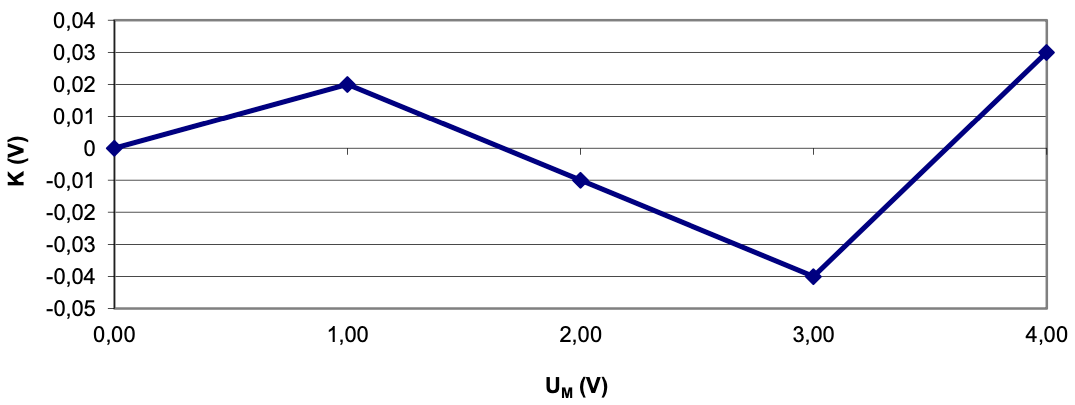
\includegraphics[width=\textwidth]{obrazky/korekcni_krivka.png}
    \caption{\label{korek_krivka}Příklad korekční křivky}
\end{figure}

\subsection*{Vstupní odpor voltmetru}
\begin{wrapfigure}{r}{0.5\textwidth}
    \vspace{-10mm}
    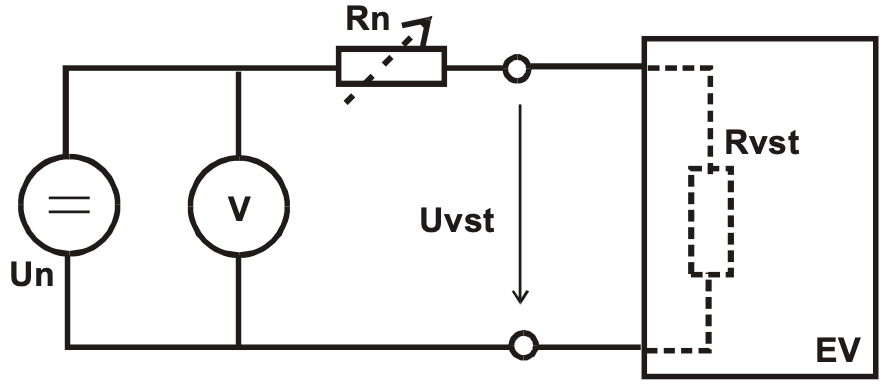
\includegraphics[width=0.5\textwidth]{obrazky/vstup_odpor.png}
    \caption{\label{vstupni_odpor}Zapojení pro měření vstupního odporu voltmetru}
\end{wrapfigure}
Vstupní odpor voltmetru je odpor, který je mezi vstupními vodiči a zemí.
Dá se jednoduše určit pomocí zdroje napětí a rezistoru se srovnatelným odporem.
\(R_{vst}=\frac{U_{vst}}{U_{n}-U_{vst}}\cdot R_n\)

\subsection{Měření AC}
Běžný frekvenční rozsah se pohybuje od \(100\-kHz\) do \(1\-MHz\).
Jeden z parametrů AC voltmetru je způsob měření efektivní hodnoty.
Buď měřený signál usměrní, změří jeho střední hodnotu a převede ji na efektivní, tato metoda je však přesná jen pro harmonický signál (střední hodnota se násobí konstantou která souvisí s konkrétním tvarem signálu a pochopitelně se proto používá nejběžnější tvar).
Druhá možnost je signál měřit pomocí definice efektivní hodnoty, která je vypočítána takto:
\begin{equation}
    U_{efe} = \sqrt{\frac{1}{T}\int_{0}^{T}U^2(t)dt}
    \label{proud_kolektoru}
\end{equation}

\subsection{Chyby měření}
Absolutní chyba měřícího přístroje se dá spočítat jako:

\begin{figure}[H]
    \begin{equation}
        |\Delta_{Px}| = |\Delta_{M}|+|\Delta_{R}| = \frac{|\delta_M\cdot X_M|+|\delta_R\cdot X_R|}{100}
    \end{equation}
    \caption{\label{proud_kolektoru}Jednotka veličiny X}
\end{figure}
Chyba měření muže vzniknout také sériovím rušením které je způsobeno především ručením se sítě (\(50\-Hz\)), toto rušení integrační AD převodníky z principu potlačují.
Potlačení rušení se dosahuje integrací v časovém úseku který je celočíselným násobkem periody měřeného napětí, pro (\(50\-Hz\)) je to \(20\-ms\).

\section{Měření}
\subsection{Použité přístroje}
\begin{itemize}
    \item Multimetr Keysight 34450A
    \item Multimetr Agilent 34401A
    \item Stabilizovaný zdroj napětí GW Instek GPD-3303S Generátor Siglent SDG2042X
    \item Odporová dekáda
\end{itemize}

\subsection{Úkol 1}
\begin{figure}[H]
    \begin{minipage}[t]{0.4\textwidth}
        \begin{table}[H]
            \vspace{-70mm}
            \begin{tabular}{|c|c|c|c|}
            \hline
                GWInstek GPD-3303S &	Agilan 34401A (etalon) &	Odchilka   \\ \hline
                \(V\)              &    \(V\)                  &	\(mV\)     \\ \hline
                 0.0               &    0.0007	               &    0.7        \\ \hline
                 1.0               &    1.0044	               &    4.4        \\ \hline
                 2.0               &    2.0042	               &    4.2        \\ \hline
                 3.0               &    3.0038	               &    3.8        \\ \hline
                 4.0               &    4.0036	               &    3.6        \\ \hline
                 5.0               &    5.0034	               &    3.4        \\ \hline
                 6.0               &    6.0044	               &    4.4        \\ \hline
                 7.0               &    7.0041	               &    4.1        \\ \hline
                 8.0               &    8.0036	               &    3.6        \\ \hline
                 9.0               &    9.0047	               &    4.7        \\ \hline
                10.0               &    10.0044                &	4.4        \\ \hline
            \end{tabular}
            \caption{\label{tab_pracovni_bod} Nastavení obvodu}
        \end{table}
    \end{minipage}
    \hfill
    \begin{minipage}[t]{0.4\textwidth}
        \tikzset{
        every pin/.style={fill=yellow!50!white,rectangle,rounded corners=3pt,font=\scriptsize},
        small dot/.style={fill=black,circle,scale=0.3}
        }
        \begin{tikzpicture}
            \begin{axis}[
                title={korekční křivka voltmetru GWInstek GPD-3303S},
                xlabel={\(U_{mer}~[V]\)},
                ylabel={\(\delta_{u}~[mV]\)},
                xmin=0, xmax=10,
                ymin=0, ymax=5,
                legend pos=north west,
            ]
            \addplot[
                color=green,
                mark=x,
                ]
                coordinates {
                        ( 0.0 ,0.7)
                        ( 1.0 ,4.4)
                        ( 2.0 ,4.2)
                        ( 3.0 ,3.8)
                        ( 4.0 ,3.6)
                        ( 5.0 ,3.4)
                        ( 6.0 ,4.4)
                        ( 7.0 ,4.1)
                        ( 8.0 ,3.6)
                        ( 9.0 ,4.7)
                        (10.0 ,4.4)
                    };
            \addlegendentry{\scriptsize}
            \end{axis}
        \end{tikzpicture}
    \end{minipage}
\end{figure}

\newpage
\subsection{Úkol 2}

\begin{figure}[H]
    \begin{minipage}[t]{0.3\textwidth}
        \paragraph{Agilent 34401A}
        \begin{itemize}
            \item \(R_n = 100\-k\Omega\) 
            \item \(U_n = 1.0032\-V\) 
            \item \(U_{vstup} = 0.9933\-V\) 
        \end{itemize}
    \end{minipage}
    \hfill
    \begin{minipage}[t]{0.7\textwidth}
        \vspace{5mm}
        \begin{equation}
            R_{vst} = \frac{U_{vst}}{U_{n}-U_{vst}}\cdot R_n = \frac{0.9933}{1.0032-0.9933}\cdot 100*10^3 = 10.033\-[k\Omega]  
        \end{equation}
    \end{minipage}
\end{figure}
Podle katalogového listu přístroje Agilent 34401A je jeho vstupní odpor \(10\-M\Omega \)\\odchylka našeho měření je tady \(33\-k\Omega\)

\begin{figure}[H]
    \begin{minipage}[t]{0.3\textwidth}
        \paragraph{Keysight 34450A}
        \begin{itemize}
            \item \(R_n = 100\-k\Omega\) 
            \item \(U_n = 1.0027\-V\) 
            \item \(U_{vstup} = 0.9928\-V\) 
        \end{itemize}
    \end{minipage}
    \hfill
    \begin{minipage}[t]{0.7\textwidth}
        \vspace{5mm}
        \begin{equation}
            R_{vst} = \frac{U_{vst}}{U_{n}-U_{vst}}\cdot R_n = \frac{0.9928}{1.0027-0.9928}\cdot 100*10^3 = 10.028\-[k\Omega]  
        \end{equation}
    \end{minipage}
\end{figure}
Podle katalogového listu přístroje Keysight 34450A je jeho vstupní odpor \(10\-M\Omega \)\\odchylka našeho měření je tady \(28\-k\Omega\)

\subsection{Úkol 3}
Pomocí generátoru jsme vytvářeli harmonický signál o amplitudě \(1\-[V]\) kterému jsme měnili frekvenci v rozsahu \(1\-[kHz]\)-\(500\-[kHz]\).\\ 
\begin{table}[H]
    \footnotesize
    \vspace{-6mm}
    \hspace{-8mm}
    \begin{tabular}{|c|c|c|c|c|c|c|c|c|c|c|}
    \hline
                        & 1 [KHz]  	& 2 [KHz]	& 5 [KHz]	& 10 [KHz]	& 20 [KHz]	& 50 [KHz]	& 100 [KHz]	& 200 [KHz]	& 350 [KHz]	& 500 [KHz] \\ \hline
    Silent SDG 2042 [V]	& 1	        & 1	        & 1      	& 1   	    & 1   	    & 1   	    & 1   	    & 1	        & 1   	    & 1         \\ \hline
    Agilan 34401A   [V]	& 1,05932	& 1,0537	& 1,05556	& 1,05977	& 1,05920	& 1,05441	& 1,04235	& 1,0158	& 0,9250	& 0,71208   \\ \hline
    Keysight 34450A [V]	& 1,0588	& 1,0589	& 1,0591	& 1,0592	& 1,0592	& 1,0576	& 1,0536	& 1,0464	& 1,0341	& 1,0186    \\ \hline
    \end{tabular}
    \caption{\label{frekvencni_rozsah} Měření frekvenčního rozsahu}
    \normalsize
\end{table}

\pgfplotsset{width=100mm,compat=1.9}
\begin{tikzpicture}
    \begin{semilogyaxis}[
        title={korekční křivka voltmetru GWInstek GPD-3303S},
        xlabel={\(U_{mer}~[V]\)},
        ylabel={\(\delta_{u}~[mV]\)},
        xmin=0, xmax=510,
        ymin=0.7, ymax=1.1,
        legend pos=south west,
    ]
    \addplot[
        color=green,
        mark=x,
        ]
        coordinates {
                ( 1   ,1.05932)
                ( 2   ,1.0537)
                ( 5   ,1.05556)
                ( 10  ,1.05977)
                ( 20  ,1.05920)
                ( 50  ,1.05441)
                ( 100 ,1.04235)
                ( 200 ,1.0158)
                ( 350 ,0.9250)
                ( 500 ,0.71208)
            };
    \addlegendentry{\scriptsize Agilan 34401A}
    \addplot[
        color=red,
        mark=x,
        ]
        coordinates {
                ( 1   ,1.0588)
                ( 2   ,1.0589)
                ( 5   ,1.0591)
                ( 10  ,1.0592)
                ( 20  ,1.0592)
                ( 50  ,1.0576)
                ( 100 ,1.0536)
                ( 200 ,1.0464)
                ( 350 ,1.0341)
                ( 500 ,1.0186)
            };
    \addlegendentry{\scriptsize Keysight 34450A}
    \end{semilogyaxis}
\end{tikzpicture}
% Přístroj Keysight 34450A má uvedený frekvenční rozsah do \(300\-[kHz]\)

\subsection{Úkol 4}
Multimetrem Keysight 34450A jsme změřili nejprve obdélníkoví (\(U_{pp} = 3\-[V]\);\(f=1\-[kHz]\)) signál a následně trojúhelníkoví (\(U_{pp} = 5\-[V]\);\(f=100\-[Hz]\))
\begin{itemize}
    \item obdélníkový signál - \(U_{EF} = 1.4850\-[V]\)
    \item trojúhelníkoví signál - \(U_{EF} = 1.4411\-[V]\)
\end{itemize}

\begin{figure}[H]
    \begin{minipage}[t]{0.7\textwidth}
        \vspace{-55mm}
        \hspace{-5mm}
        Elektivní hodnota obdélníkového signálu (\(U_{pp} = 3\-[V]\);\(f=1\-[kHz]\)) je:
        \\
        \(
            U_{EF} = \sqrt{\frac{1}{T}(\int_{0}^{T}U^2(t)dt} = \\
            = \sqrt{\frac{1}{\frac{1}{1000\-[Hz]}}\Biggl(\int_{0}^{\frac{\frac{1}{1000\-[Hz]}}{2}}1.5^2dt+\int_{0}^{\frac{\frac{1}{1000\-[Hz]}}{2}}(-1.5)^2dt\Biggl)} = \\\
            = \sqrt{1000\cdot2\int_{0}^{0.0005}2.25dt} =\\
            = \sqrt{1000\cdot2\cdot\bigr[2.25t \bigr]_{0}^{0.0005}} = \sqrt{1000\cdot2\cdot0.001125} = 1.5\-[V]
        \)
        \\
        Měření tedy oproti teorii vykazuje odchylku \(15\-[mV]\)
    \end{minipage}
    \hfill
    \begin{minipage}[t]{0.4\textwidth}
        \hspace{-5mm}
        \pgfplotsset{width=\textwidth,compat=1.9}
        \begin{tikzpicture}
            \begin{axis}[
                title={obdelníkoví signál},
                xlabel={\(t~[ms]\)},
                ylabel={\(U~[V]\)},
                xmin=0, xmax=2.5,
                ymin=-2, ymax=2,
                legend pos=south west,
            ]
            \addplot[
                color=green,
                ]
                coordinates {
                        (0   ,-1.5)
                        (0.5 ,-1.5)
                        (0.5 , 1.5)
                        (1   , 1.5)
                        (1   ,-1.5)
                        (1.5 ,-1.5)
                        (1.5 , 1.5)
                        (2   , 1.5)
                        (2   ,-1.5)
                        (2.5 ,-1.5)
                    };
            \end{axis}
        \end{tikzpicture}
    \end{minipage}
\end{figure}

\begin{figure}[H]
    \begin{minipage}[t]{0.7\textwidth}
        \vspace{-60mm}
        \hspace{-5mm}
        Elektivní hodnota trojúhelníkového signálu (\(U_{pp} = 5\-[V]\);\(f=100\-[Hz]\)) je: \\
        \(
            U_{EF} = \sqrt{\frac{1}{T}(\int_{0}^{T}U^2(t)dt} = \\
            = \sqrt{\frac{1}{\frac{1}{100\-[Hz]}}\Biggl(\int_{0}^{\frac{\frac{1}{100\-[Hz]}}{2}} (-2.5+1000t)^2 dt+\int_{\frac{\frac{1}{100\-[Hz]}}{2}}^{\frac{1}{100\-[Hz]}} (7.5-1000t)^2 dt\Biggl)} = \\
            = \sqrt{100\cdot\Biggl(\int_{0}^{0.005} 6.25-5000t+10^6t^2 dt + \int_{0.005}^{0.01} 56.25-15000t+10^6t^2 dt\Biggl)} = \\
            = \sqrt{100\cdot\Bigr(\bigr[6.25t-2500t^2+\frac{10^6t^3}{3} \bigr]_{0}^{0.005} + \bigr[56.25t-7500t^2+\frac{10^6t^3}{3}\bigr]_{0.005}^{0.01}\Bigr)} = \\
            = \sqrt{100\cdot(0.01042+0.01042)} = 1.4436\-[V]
        \)
        \\
        Měření tedy oproti teorii vykazuje odchylku \(2.5\-[mV]\)
    \end{minipage}
    \hfill
    \begin{minipage}[t]{0.4\textwidth}
        \hspace{-5mm}
        \pgfplotsset{width=\textwidth,compat=1.9}
        \begin{tikzpicture}
            \begin{axis}[
                title={obdelníkoví signál},
                xlabel={\(t~[ms]\)},
                ylabel={\(U~[V]\)},
                xmin=0, xmax=40,
                ymin=-3, ymax=3,
                legend pos=south west,
            ]
            \addplot[
                color=green,
                ]
                coordinates {
                        (00   ,-2.5)
                        (10   , 2.5)
                        (20   ,-2.5)
                        (30   , 2.5)
                        (40   ,-2.5)
                        (50   , 2.5)
                    };
            \end{axis}
        \end{tikzpicture}
    \end{minipage}
\end{figure}

\subsection{Úkol 5}
Jako zdroj rušivého signálu smě použili zdroj Siglent SDG2042X 


\end{document}
